\documentclass{article}

% if you need to pass options to natbib, use, e.g.:
%     \PassOptionsToPackage{numbers, compress}{natbib}
% before loading neurips_2019

% ready for submission
% \usepackage{neurips_2019}

% to compile a preprint version, e.g., for submission to arXiv, add add the
% [preprint] option:
%     \usepackage[preprint]{neurips_2019}

% to compile a camera-ready version, add the [final] option, e.g.:
\usepackage[]{neurips_2019}

% to avoid loading the natbib package, add option nonatbib:
%     \usepackage[nonatbib]{neurips_2019}

\usepackage[utf8]{inputenc} % allow utf-8 input
\usepackage[T1]{fontenc}    % use 8-bit T1 fonts
\usepackage{hyperref}       % hyperlinks
\usepackage{url}            % simple URL typesetting
\usepackage{booktabs}       % professional-quality tables
\usepackage{amsfonts}       % blackboard math symbols
\usepackage{nicefrac}       % compact symbols for 1/2, etc.
\usepackage{microtype}      % microtypography
\usepackage{textgreek}
\usepackage{graphicx}

\title{Final Report: Malmo Minecraft Mazerunner}

% The \author macro works with any number of authors. There are two commands
% used to separate the names and addresses of multiple authors: \And and \AND.
%
% Using \And between authors leaves it to LaTeX to determine where to break the
% lines. Using \AND forces a line break at that point. So, if LaTeX puts 3 of 4
% authors names on the first line, and the last on the second line, try using
% \AND instead of \And before the third author name.

\author{%
  Jordan Choi \\
  Yixuan Li \\
  Joshua Lu \\
}

\begin{document}

\maketitle

\begin{abstract}
  Our project is to develop and train an agent that can guide our Minecraft user from the beginning of a maze to the end. The main idea is to create an agent that is capable of learning and familiarizing itself in different environments and then make the most optimal decision at every move to find the best overall combination of actions to solve the maze. The agent is first placed in a predetermined starting position and its goal is to reach the endpoint whose location is unknown to the agent and is up to it to find that diamond or gold block that represents the ending point. The agent will decide between a combination of simple actions such as moving as well as complicated actions like jumping in order to reach the endpoint. 
  \\ \\ We have accomplished two of the three goals we had set out for our project. Firstly, our minimum goal was to accomplish simple movement from the start point to the end point of a basic maze (small in size and not difficult to navigate). Ever since the beginning, we have been using the deep Q-learning approach to simulate reinforcement learning and the agent showed capability in solving basic mazes efficiently by finding the fastest path from start to the end of the maze. Our realistic goal was to include the more complicated action of jumping. We wanted the agent to be able to solve more complicated mazes where there were multiple routes to the end goal but there was one specific route that would be more optimal than the rest. We wanted our ambitious goal to include more complex actions such as the ability to build and manipulate the map in order to let the agent create its own optimal route to the destination. As we worked on our realistic goal, we realized the complexity of adding the jump action as well as working with more complex maps, so we were not able to reach our ambitious goal and decided rather to commit our time to optimizing our agent and experimenting with different approaches in regards to our realistic goal.


\end{abstract}

\section{Introduction}

The goal of our project is to train our agent to be able to navigate a maze from beginning to end. We want our agent to be able to learn to direct the user through varying obstacles based on its experience amassed from reinforced learning. What separates an artificial intelligence agent from just a well-coded maze solver is its ability to learn and adapt and make good decisions in unknown environments. We wanted to create an agent that doesn't just solve mazes through countless repeated runs, where eventually the agent will have touched on every part of the map and discovered a route to the finish line. We wanted to create an agent that is efficient and can make smart decisions at every move to determine the optimal solution in any unfamiliar maze without running a ridiculous amount of episodes. We decided to implement a deep Q-learning approach because it addresses both of these demands. Q-learning is interesting in that it implements randomization during the testing phase to force the algorithm to deal with unpredictable states and require a degree of generalization when it comes to decision making. This answers our problem as implementing Q-learning allows our agent to rely on reinforced learning to build up enough experience to make smart decisions in order to discover the optimal path to solve the maze. We briefly played around with different approaches in regards to the observation mechanism used by our agent. We began by using grid-based observations with tools provided by the Malmo platform which worked seamlessly. We also decided to try frame-based observations where each frame of the game represented a different state and was a visually dependent approach. We ultimately decided to stick with grid-based observations as it was more in line with our approach towards the project and allowed us to focus more efforts into optimizing our agent and experimenting with different approaches in regards to our underlying algorithm. 

\section{Background}

Our project is set in Minecraft, a video game that allows a player to control an agent to explore and craft in the world, and build complicated structures. We are using Project Malmo, an open source platform built on Minecraft for artificial intelligence experimentation to help the agent act and sense within the Minecraft environment. We are also using its provided Q-learning library. 

\section{Problem Statement}

The agent first starts at a predetermined starting block in a maze that also has a goal block. The maze has redstone blocks for “walls” and quartz blocks as possible paths for the agent to take. The agent has no information on the environment at the start but can slowly figure out its environment as it explores to find and reach the goal state. \\
The agent was given five actions: the agent can move forwards, backwards, turn left, turn right, or jump in a direction. We used Malmo to control the agent’s movement and actions. Furthermore, we assigned the algorithm this reward system:

\begin{itemize}
    \item -1 for each move in a direction
    \item -1 for each jump
    \item -100 for dying
    \item +500 for getting to the gold block
    \item +1000 for getting to the diamond block
    \item $-10  \times $(distance from goal) for each episode
\end{itemize}
The minimum goal of our project was to accomplish simple movement from the start point to the end point in a basic maze. The first milestone was using only back and forth movement and then in the second milestone, use a combination of front, back, left, and right movement to navigate to the end point. We constructed a very simple maze for testing to make sure our agent would be able to learn the maze and navigate to the diamond block which indicated success. The realistic goal saw the addition of the jumping action in order for the agent to explore and discover three dimensional paths that may lead to the end goal. Our milestone was to teach the agent to use the jump action when it was more efficient to do so rather than settling with the longer path that can be reached through the four original basic movements. We purposely created maps that would require the agent to use the jump action in order to use that optimal path in order to test the agent’s decision making ability, as well as ability to discover the map. Our ambitious goal included more complex actions such as the ability to build and manipulate the map in order to let the agent create its own optimal path to the destination. We had envisioned for the milestone to be the ability to construct bridges or paths to cross over sections of the maze that were not possible before and not meant for the agent to perform using traditional actions. Ultimately, the ambitious goal was not completed given the time constraint and context of this project class.

\section{Method}

Our agent follows the Markov Decision Process to determine the most efficient path. At each step, the agent examines and interacts with the environment and receives a certain reward. With each action, the agent receives a reward that depends on all previous states and actions it took to get to the current state. Thus, the agent chooses the appropriate action for its current state depending on actions in previous states. \\
Now given we know the expected reward of each action at every step, we use Q-learning, to generate the maximum total reward, which in Q-learning is called the Q-value. 

\begin{center}
    \[Q(s,a) = r(s,a) + \gammma \max_{a} Q(s', a)\]
    \center Figure 1: Markov Decision Process: Reinforcement Learning
\end{center}

The Q-value we calculate comes from being at the state “s” at which we will make the action “a”. To get Q, we will calculate the immediate reward of making action “a” at state “s”, shown by “r(s,a).” We will add this with the highest Q-value possible from the next state s’. We include the value of gamma as it controls how much influence the future reward has by either increasing or decreasing it based on what value we assert gamma as. \\
We also implement an \textepsilon -greedy policy to avoid getting stuck in the local minimum if it only chooses actions that optimize the Q-function. The \textepsilon -greedy method will either choose the action with the highest q-value or a random action. This decision is made randomly and is based on the value of epsilon where the value of \textepsilon is purposely set so that we lean towards using random actions at first, but as training progresses, become more reliant on maximum Q-values instead. With this policy, the agent will randomly choose an action that is not optimal so the agent has the chance to explore the environment more at the off chance that the true optimal path is elsewhere and prevent overfitting. To further enhance the influence and effectiveness of the epsilon-greedy method, we explored the concept of Exploration vs Exploitation through using epsilon decay. When our first set of episodes were being run on generated mazes, we adjusted the epsilon to a higher value. A higher epsilon showcased exploration as there was a higher probability that the agent would make a random choice which allowed for the agent to explore different parts of the map, effectively mapping out what the environment was like. As episodes reached a consistent higher count, we decreased the epsilon to a smaller value to allow for exploitation rather than exploration. With the agent less likely to make random moves, it focused on the results of the Qtable, relying more on reinforced learning to follow the optimal string of actions to reach the endpoint. This would reinforce the optimal route the agent had discovered through exploration in earlier episodes. \\
Furthermore, as mentioned in our problem statement, we also incorporated a distance penalty into our algorithm that accounted for the steps taken by the agent in order to reach the end goal. With the distance penalty being a negative value, the more steps we took in our overall path, the smaller the overall reward value and ultimately the less valuable that path is to our decision making process of creating an efficient route to the end. 


\section{Experiments}

We first designed a map to see whether model would learn a simple map with a basic path get towards the goal. This was to see whether the Q-learning algorithm was properly inserting value into the table. To see the Q-learning process in action, we explicitly designed two maps that would demonstrate whether the model would find the most optimal path. The first map had two goal nodes with two simple paths with one path towards a gold block and one longer path towards a diamond block. The second map had one goal node towards a diamond block with two paths. One that required jumping that would ultimately take a shorter number of actions to get towards the goal and one that was much longer that did not require jumping. Our final map was a more ambitious map that incorporated multiple floors that required jumping, multiple goal nodes, and multiple paths. The goal of this map was to really test the model, see how it would behave, and see if it would be able to find the most optimal path. 

\section{Results}

Results were measured as the cumulative reward for each episode over the number of episodes. An expected result should show a positive relationship between the two variables. At first, the graph should initially dip into the negative region as the agent is penalized for movements and deaths. As the model continues exploring and exploiting, the model should eventually increase and peak at the optimal solution. Once the model peaks, slight deviations should show a scatter of points under the peak as a result of a positive non-zero epsilon value. \\
The first map reflects the expected outcome of the graph without any unforeseen trends. As the first map is a simple path towards a goal, the agent finds the optimal path relatively early in training showing an initial negative trend and then switching to a positive trend after discovering the goal node for the first time. \\
\begin{center}
    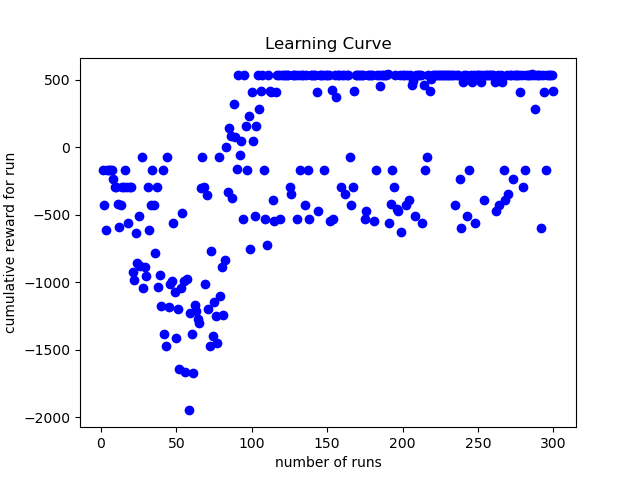
\includegraphics[scale=0.39]{NeuRIPS2019/images/1_simple.png}
    \center Figure 2: Map 1 Plot
\end{center}

In the second map, the agent was quickly able to find the gold block early on as it was the very close to the starting node. This is reflected in the early trend line of consistent rewards of 220. The agent continues exploring and was able to find a more optimal path soon after discovering the gold block that the diamond block was more optimal and the trend quickly shifted, favoring a higher reward. This is reflected in the greater concentration of plots in the 800 range. \\
\begin{center}
    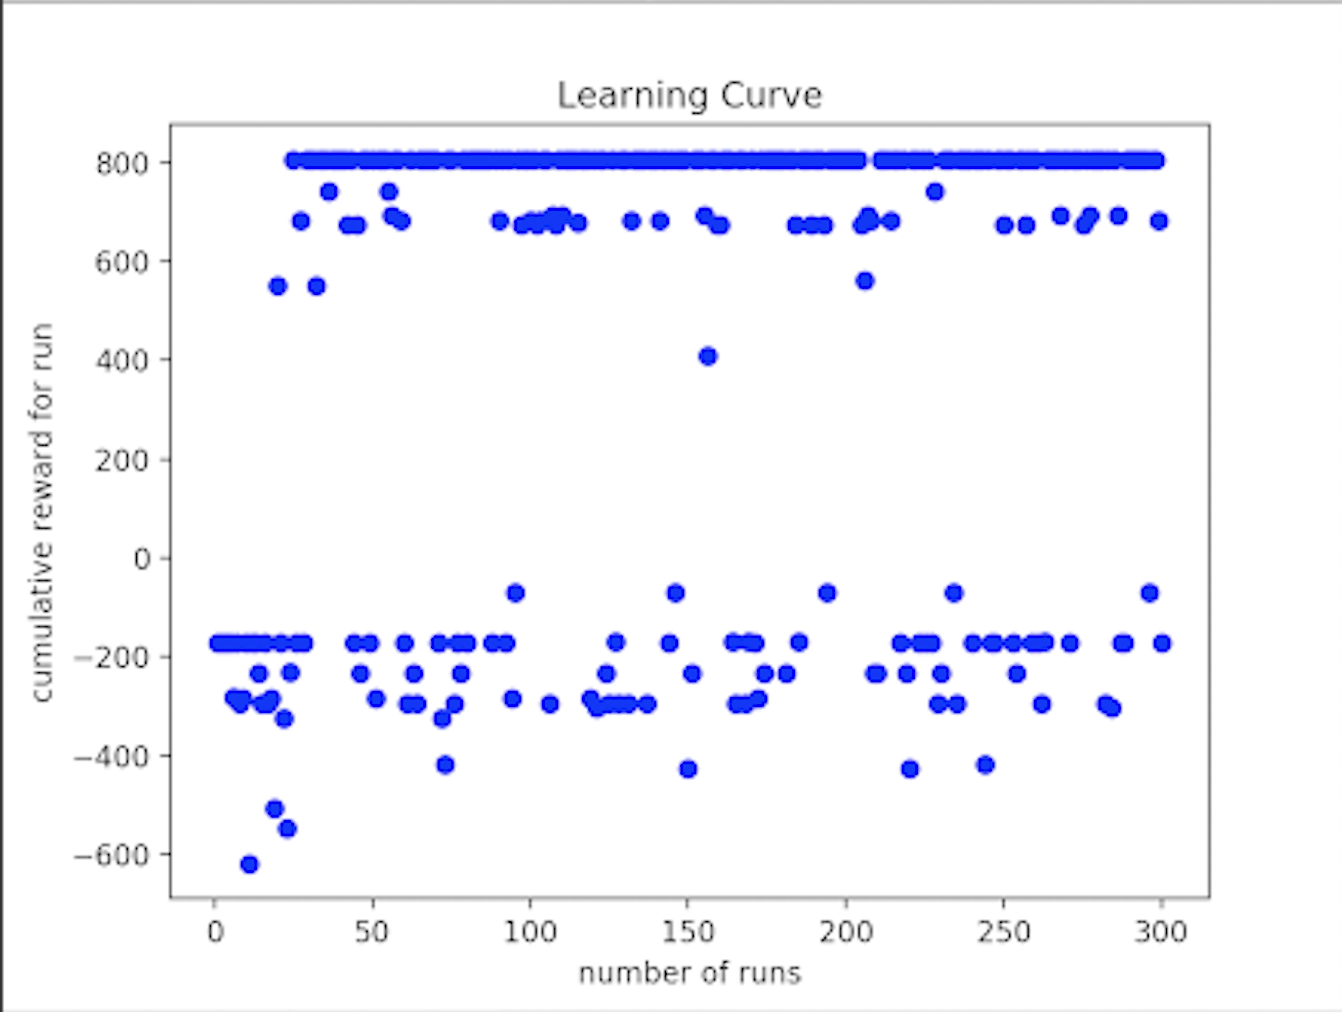
\includegraphics[scale=0.35]{NeuRIPS2019/images/3_diamondgold_3.png}
    \center Figure 3: Map 2 Plot
\end{center}

A similar trend from the second map, follows in the third map albeit slightly less obvious at first. At first, the agent learns how to reach the goal node without jumping however, it later discovers that jumping over a block would produce a more optimal, shorter path due to the cost associated with each step taken. The graph reflects this trend rather subtly between episodes 60 and 120 versus episodes 120 to the end. The first half shows a slightly smaller reward of roughly 7 steps compared to the slightly greater second half. This is a direct result of the number of steps the agent took to move around a hazard versus saving those steps by jumping over the hazard. Exploration of the map resulted in expected trends both before the agent began consistently discovering a path to the goal and after the agent discovered a path to the goal node\\
\begin{center}
    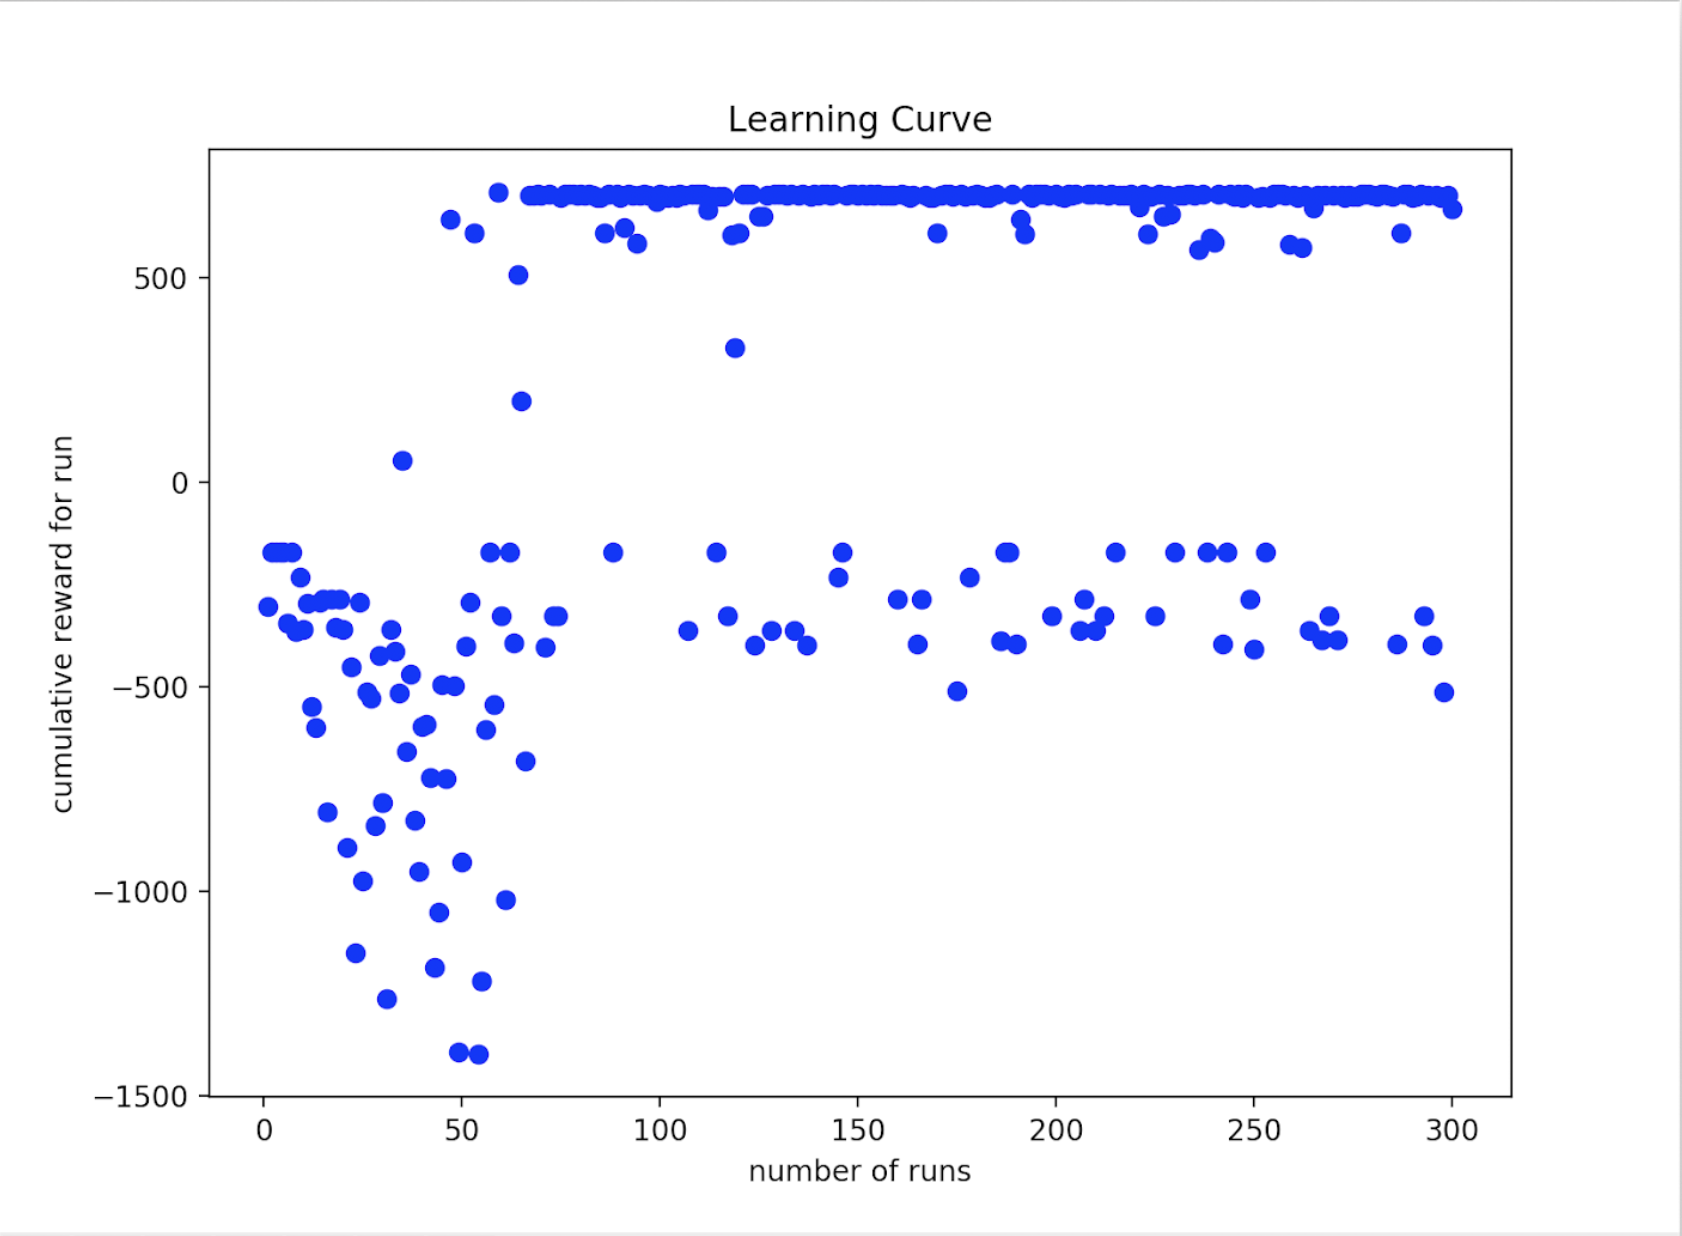
\includegraphics[scale=0.30]{NeuRIPS2019/images/4_jump.png}
    \center Figure 4: Map 3 Plot
\end{center}

The final map we tested involved a heavily more ambitious path to reach the optimal goal node. It was slightly larger and had multiple floors with multiple goal states. This map was created with the intention of placing the agent under more realistic conditions and stresses in the world of Minecraft. The resulting graph had the expected trends of exploration plots due to the epsilon being greater than zero however, the two concurrent trend lines of the graph were difficult to interpret. The lines represented the ending states of the agent learning how to reach the lesser reward of the gold block however, it pointed out different paths of reaching the gold block as well as pointing out a bug within our code. \\
In Malmo, as soon as the agent touches the block with any part of its body, the goal is considered reached and the episode terminates. In the -485 cumulative reward range, the agent had learned to reach the goal node by climbing stairs and walking to the goal node. This state was further by roughly 16 blocks from the most optimal diamond block goal of which we were using to calculate the \verb|distance_from_goal| value. In the 10 cumulative reward range, the agent had learned to reach a block one floor beneath the goal we had intended for and jumped to touch its head to the goal; an unforeseen solution to reach the goal. This state was further by roughly 10 blocks from the most optimal goal node. This discrepancy of roughly 6 blocks explains the two trends when calculating the cumulative rewards of $-10 \times 6$ as found in the reward system. The agent had just began favoring the more optimal solution of touching its head to reach the goal node before the limit to the number of episodes was reached. We hypothesize that the agent would continue to learn the map after significantly more episodes to reach the more optimal goal state of the diamond block due to the nature of the agent having many more states to explore than those of the previous maps.
\begin{center}
    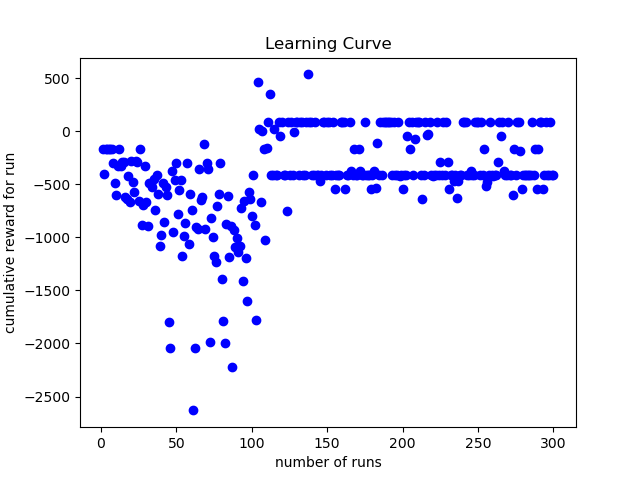
\includegraphics[scale=0.40]{NeuRIPS2019/images/5_amibtious.png}
    \center Figure 5: Map 4 Plot
\end{center}


\section*{References}
\small
[1] Choudhary, Ankit, et al. “\emph{Introduction to Deep Q-Learning for Reinforcement Learning (in Python).}” Analytics Vidhya, 6 May 2019, www.analyticsvidhya.com/blog/2019/04/introduction-deep-q-learning-python/.

[2] Ossenkopp, Philip, et al. “Reinforcement Learning – Part 1: Introduction to Q-Learning.” 
Novatec, 13 Feb. 2020, www.novatec-gmbh.de/en/blog/introduction-to-q-learning/. 

[3] Violante, Andre. “Simple Reinforcement Learning: Q-Learning.” Medium, Towards Data Science, 1 July 2019, towardsdatascience.com/simple-reinforcement-learning-q-learning-fcddc4b6fe56.

\end{document}
